Im Rahmen dieser Arbeit wird ein Bildschirmtisch zur Projektion dreidimensionaler Inhalte verwendet, welcher Multi-Touch Eingaben erlaubt. Gegenüber handgehaltenen Geräten, wie Smartphones, oder Tablets, bietet dieser eine weit größere Interaktionsfläche. Diese begünstigt, wie in Abschnitt \ref{sec:mehrbenutzer_vr_systeme} beschrieben, die kollaborative Arbeit in einem Mehrbenutzerszenario. Die meisten multi-touch gesteuerten Eingabegeräte ordnen alle erkannten Fingerpositionen und deren Bewegung derselben Geste zu. Bei gleichzeitiger Bedienung durch mehrere Nutzer, können nach diesem Ansatz leicht Eingabekonflikte entstehen. Um dem Problem entgegenzuwirken ist ein System erforderlich, welches Aussagen über die hierarchische Zuordnung der Eingabepositionen treffen kann.
\\\\
Hierzu wird in dieser Arbeit die von Ewerling et al. entwickelte Finger und Hand Tracking Implementierung, auf Grundlage des Maximally Stable Extremal Regions (MSER) Algorithmus verwendet \cite{matas:2004, ewerling:2012}. Der theoretische Ansatz dieser Lösung wird in Abschnitt \ref{sec:maximally_stable_extremal_regions} vorgestellt. Abschnitt \ref{sec:technische_voraussetzungen} beleuchtet die technischen Voraussetzungen zur Umsetzung des Multi-Touch Tisches, gefolgt von einem Überblick über die softwareseitige Integration des  MSER Trackings in das genutzte Applikationsframework in Abschnitt \ref{sec:implementierung_mser}. Zuletzt werden die Vorteile und Limitierungen des Systems in Abschnitt \ref{sec:diskussion_mser} diskutiert.


\section{Maximally Stable Extremal Regions}
\label{sec:maximally_stable_extremal_regions}

\begin{figure}
	\begin{center}
		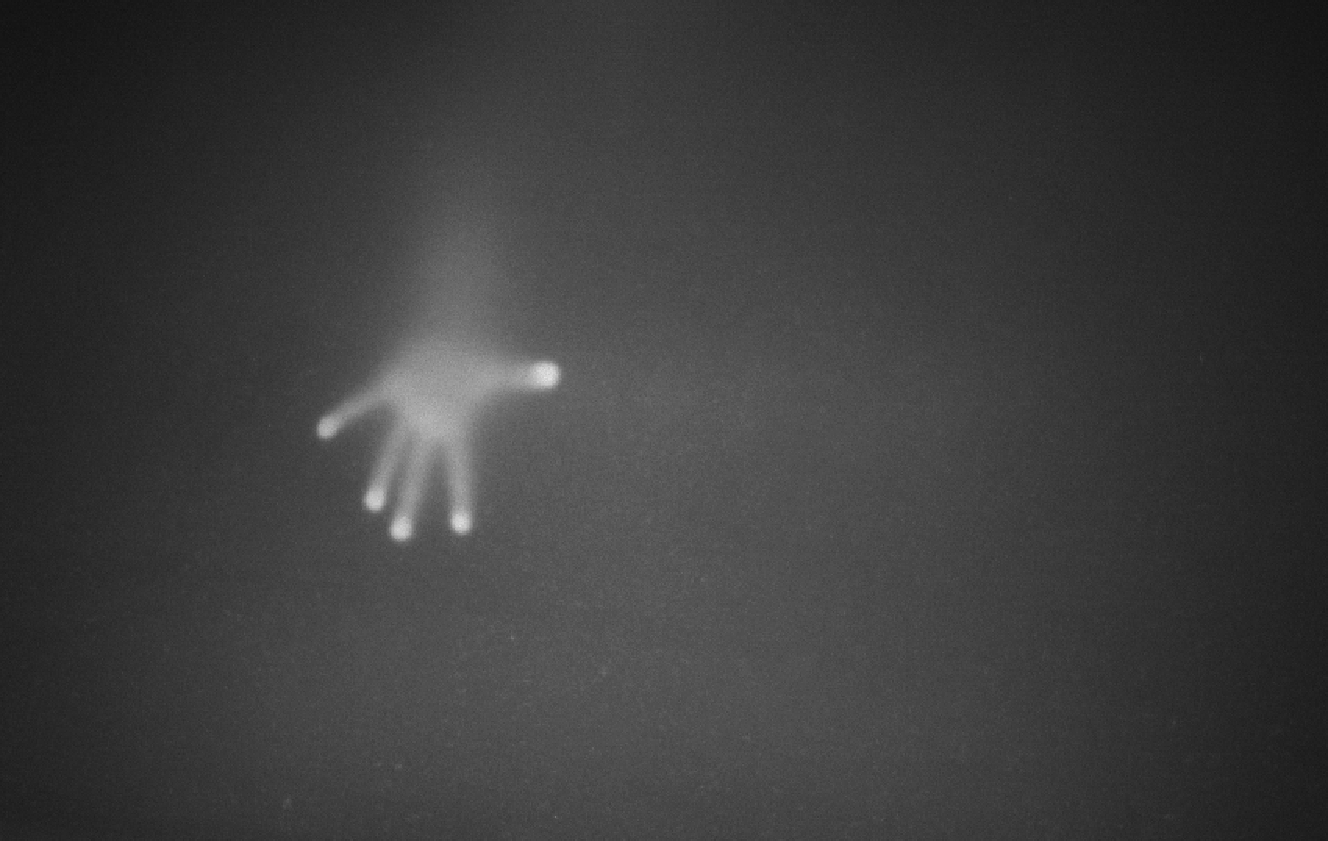
\includegraphics[width=12cm]{img/mser_1.pdf}
	\end{center}
	\caption{Das von der Infrarot Kamera eingefangene Rohbild zur Toucherkennung.}
	\label{fig:mser_1}
\end{figure}

Maximally Stable Extremal Regions ist ein Ansatz entwickelt von Matas et al. zur Auswertung von Bildreihen bei der photogrammetrischen Stereo-Rekonstruktion \cite{matas:2004}. Hierbei sollen vor allem eigenschaftsbezogene Korrespondenzen zwischen Stereobildpaaren mit unterschiedlichem Blickpunkt gefunden werden. Ewerling et al. nutzen diese Erkenntnisse zur Erkennung von Fingerspitzen auf dem Bildschirm \cite{ewerling:2012}. Es erfolgt dabei außerdem eine Zuordnung von Fingern zu Händen durch den \emph{MSER Component Tree}.  Dieses Verfahren ist motiviert durch die visuelle Wahrnehmung des Hand- und Armschattens auf den Bildern, welche durch Tracking mit diffuser Infrarotbeleuchtung erfasst werden (siehe Abbildung \ref{fig:mser_1}).

Extremal Regions (ER) werden als geschlossene Gruppe von Pixeln bezeichnet, welche entweder eine höhere oder eine niedrigere Farbintensität als umliegende Bildpunkte aufweisen. Die ER $R_i$ ist eine Maximally Stable Extremal Region, wenn $R_i$ eine anderen RE ($R_{i-1}$) umschließt und es eine umschließende ER ($R_{i+1}$) für $R_i$ gibt. Es muss folglich $R_{i-1} \subset R_i \subset R_{i+1}$ gelten. Außerdem muss das Stabilitätskriterium ($s_\Delta(i)$) für $i$ ein lokales Minimum erreichen. Folgende Formel beschreibt die Berechnung von $s_\Delta(i)$:
\\\\
$s_\Delta(i) = \frac{ |R_{i+\Delta}| - |R_{i-\Delta}| } { |R_i| }$
\\\\ 
,wobei $\Delta$ eine durch den Anwender definierte Konstante ist.
\\\\
Ewerling et al. nutzen einen erweiterten Ansatz zur Erkennung der MSER in linearer Zeit, nach dem Vorbild von Nistér et al. \cite{nister:2008}. Bei der direkten Verwendung der Methode von Nistér et al. ergibt sich eine hierarchische Struktur zur Beschreibung  aller gefundenen MSER, basierend auf dem Stabilitätskriterium. Genannte Struktur wird als \emph{Component Tree} bezeichnet. Die Konstruktion dieses Component Trees sei jedoch nach Ewerling et al. unvollständig im Hinblick auf für die Beschreibung der Finger-Hand-Relation wichtige ER. Der erweiterte Algorithmus wurde daher entwickelt, um alle verfügbaren ER zu analysieren.
\\\\
Anhand der ER im Component Tree erfolgt die Ableitung der Fingerpositionen und deren Handzuordnung. Hierfür definieren Ewerling et al. zwei grundlegende Regeln:

\begin{enumerate}
\item Die dunkelste und gleichzeitig größte gefundene ER ist der Wurzelknoten des Component Trees
\item Für alle Kind-Eltern Beziehungen in der Struktur gilt, dass die Kindknoten kleiner sind und eine höhere Farbintensität aufweisen
\end{enumerate}

\begin{figure}
	\begin{center}
		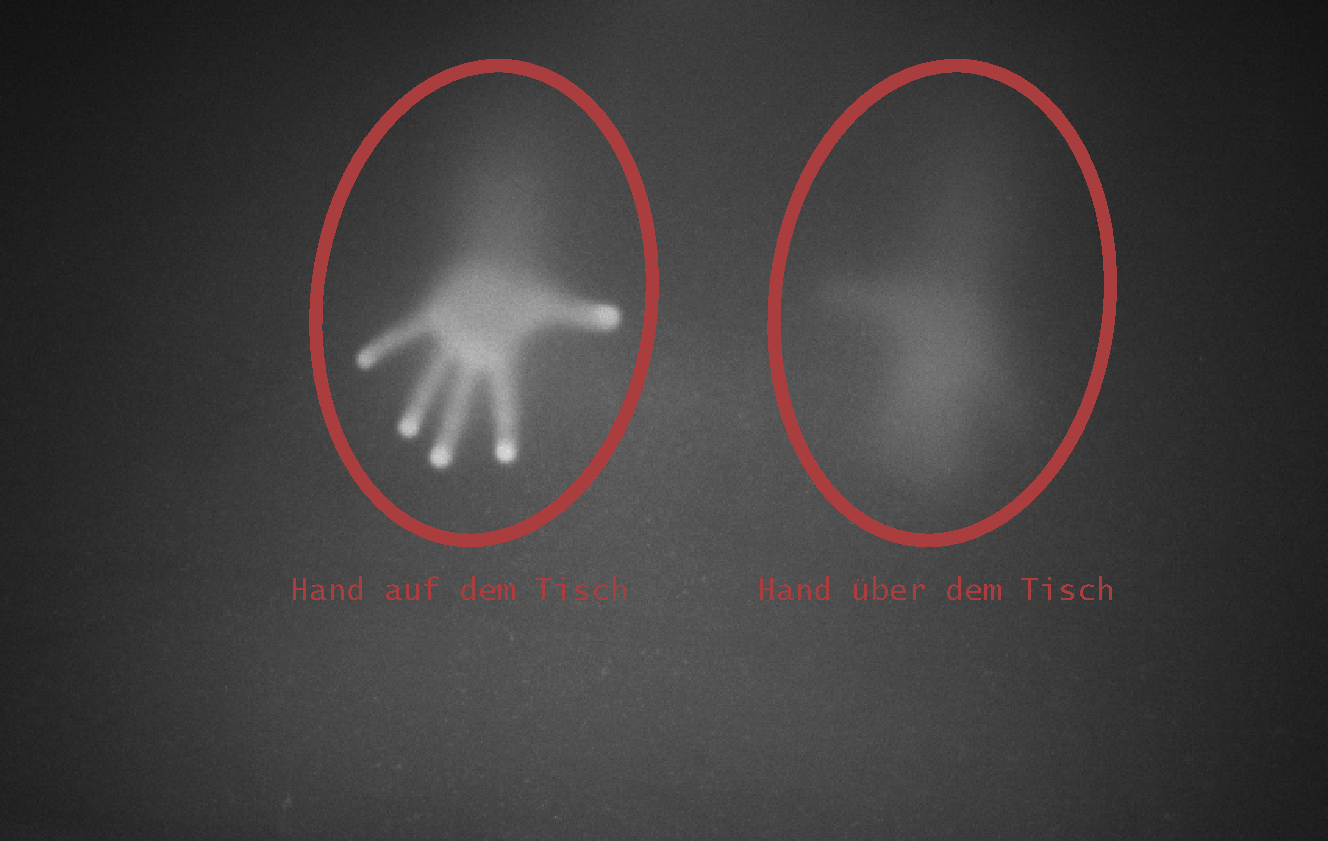
\includegraphics[width=12cm]{img/mser_2.pdf}
	\end{center}
	\caption{Die Helligkeit naher Objekte ist im Infrarot Bild höher als bei weiter entfernten.}
	\label{fig:mser_2}
\end{figure}

Wie in Abbildung \ref{fig:mser_2} zu erkennen ist, kreieren Objekte in naher Distanz zum Bildschirm eine hellere ER als weiter entfernte. Nach den gelisteten Kriterien können folglich nur Blattknoten des Baumes Fingerspitzen sein. Um eine robuste Analyse zu erreichen, werden vermeidliche Kandidaten in der untersten Ebene des Baumes auf typische visuelle Eigenschaften von Fingeraufsetzpunkten getestet. Hierzu zählen das Prüfen auf runde Form und eine definierte Durchschnittsgröße der erkannten Fingerregion. Die Zuordnung der gefundenen Fingerspitzen zu Händen erfolgt über ein hierarchisches Clustering der Knoten im Component Tree.


\section{Technische Voraussetzungen}
\label{sec:technische_voraussetzungen}

Für die technische Umsetzung des in Abschnitt \ref{sec:maximally_stable_extremal_regions} beschriebenen MSER Systems im Kontext der Multi-Touch Erkennung wird in unserem Labor ein rückseitiges, diffuses Infrarotbeleuchtungssetup genutzt. Hierbei wird eine diffuse Infrarot emittierende Lichtquelle unterhalb des Bildschirmtisches angebracht. Ein Spiegel lenkt das Licht senkrecht auf eine matte und lichtdurchlässige Projektionsfläche. Das von dieser Ebene reflektierte Licht wird durch den Spiegel gelenkt und von einer Infrarotkamera zur weiteren Verarbeitung aufgenommen. Abbildung \ref{fig:table_setup} visualisiert das beschriebene Setup.

\begin{figure}
	\begin{center}
		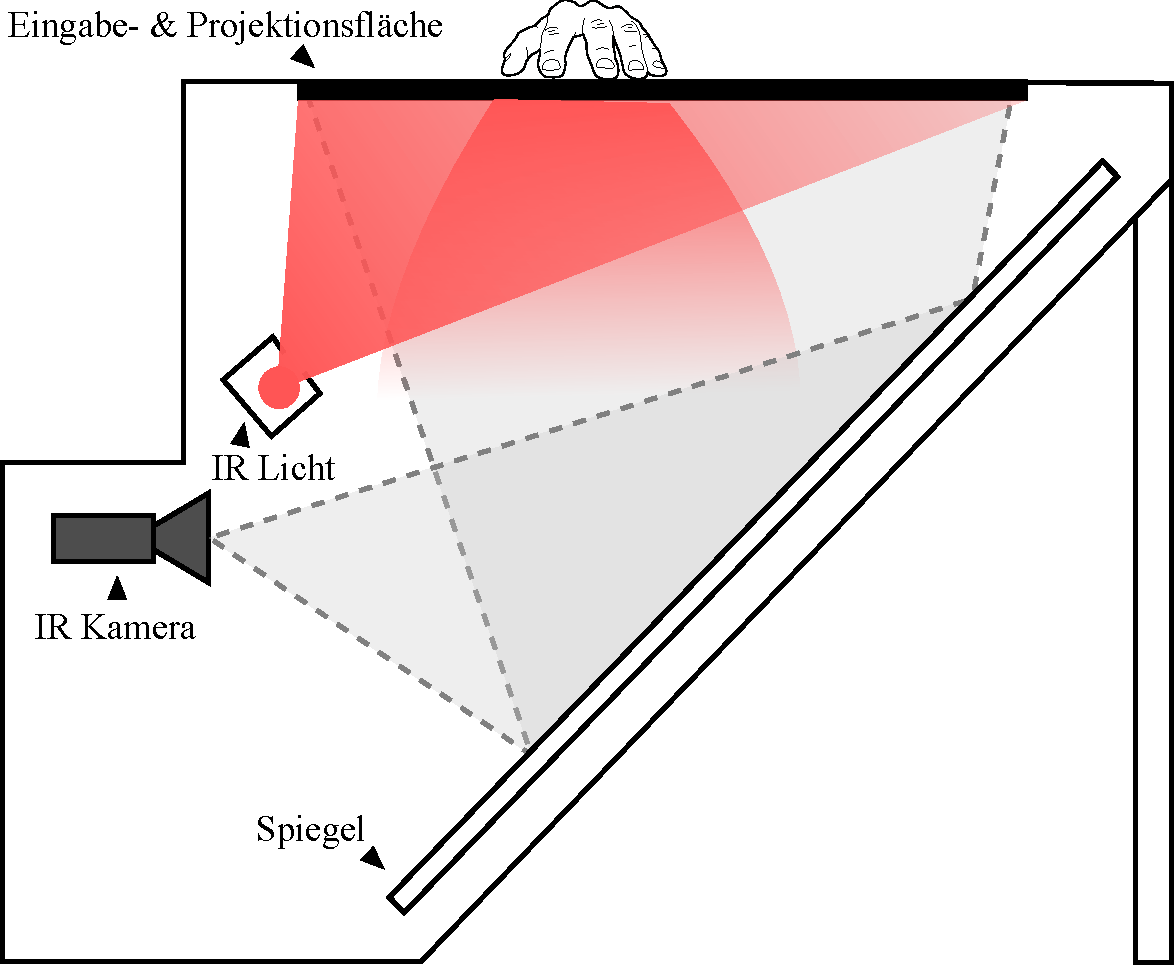
\includegraphics[width=8cm]{img/table_setup.pdf}
	\end{center}
	\caption{Das im Labor verwendete Hardware Setup zum Tracking von Touch Eingaben.}
	\label{fig:table_setup}
\end{figure}

Die Genauigkeit des Systems kann durch infrarotes Umgebungslicht, wie beispielsweise Anteile der Sonnenstrahlung, oder andere im Arbeitsraum befindliche Trackingsysteme, gestört werden. Ewerling et al. schlagen daher eine hochfrequente Modulation der Beleuchtung nach Moeller und Kerne vor \cite{ewerling:2012, moeller:2012}.  Nicht-uniforme Lichtintensität entlang der Tischfläche kann ebenfalls zu Problemen bei der Bildanalyse führen. Diese können zwar durch Filterverfahren abgeschwächt, jedoch nicht vollständig beseitigt werden. Eine gleichmäßige Ausleuchtung der Projektionsebene ist demnach ausschlaggebend für eine akkurate Evaluation der Kamerabilder.


\section{Implementierung}
\label{sec:implementierung_mser}
Es existiert eine Anbindung des MSER Algorithmus zur Touch Erkennung, an das am Lehrstuhl entstandene Applikationsframework Avango\footnote{http://www.avango.org/}. Die analysierten Eingabedaten werden basierend auf dem TUIO Protokoll\footnote{http://www.tuio.org/} an die Anwendung gesendet.
\\\\
In Abschnitt \ref{subsec:tuio_touch_protokoll} wird eine Übersicht über die mit dem TUIO Protokoll bereitgestellten Datenstrukturen gegeben. Abschnitt \ref{subsec:umgang_mit_jittering} beschreibt das Auftreten von Jittering bei der Eingabeerkennung und wie mit diesem Problem umgegangen werden kann.


\subsection{TUIO Touch Protokoll}
\label{subsec:tuio_touch_protokoll}

TUIO ist ein von Kaltenbrunner et al. entwickeltes Protokoll, welches speziell für den Umgang mit berührbaren Tabletop Eingabeschnittstellen kreiert wurde \cite{kaltenbrunner:2005}. Nach der Auswertung der Eingabepositionen durch den MSER Algorithmus, füllt die Protokollkommunikation verschiedene Stations im Avango Daemon mit den ermittelten Daten. Es existieren zwei Stationstypen. Der Erste hält Informationen über einen jeweiligen Finger. Dies beinhaltet eine normalisierte \emph{Fingerposition}, die zugewiesene \emph{SessionID}, LIST ALL PARAMETERS. Ein weiterer Stationstyp ist für die Verwaltung handspezifischer Details verantwortlich. Hierzu gehören die \emph{SessionID} der Hand, eine Liste von \emph{FingerSessionIDs} der zugewiesenen Finger, LIST ALL PARAMETERS.
\\\\
Eine Abbildung dieser Struktur ist nach dem Feldcontainer Konzept, welches Avango bereitstellt, in der Applikation umgesetzt. Für jeden der Stationstypen existiert demnach eine Klasse, welche durch Update der Station aktualisierte Eingabewerte für die Anwendung verfügbar macht. Die nachfolgende Abbildung XX zeigt den Aufbau der Klassen \emph{TUIOFinger} und \emph{TUIOHand}.


\subsection{Umgang mit Jittering}
\label{subsec:umgang_mit_jittering}

Die Verfolgung der Bewegung von Eingabepunkten basiert auf der Auswertung von Bilddaten. Hierbei ist die Präzision der Positionsermittlung an die Genauigkeit des MSER Algorithmus, sowie die Auflösung der Bilder gebunden. Infolgedessen können, selbst bei Auflegen eines Fingers ohne Positionsverschiebung, variierende Eingabepositionen entstehen. In einer Visualisierung der Eingabeposition, äußert sich dieser Zusammenhang als Zittern (Jittering) der Darstellungsgeometrie.
\\\\
Jittering kann bei Anwendung der Eingabe auf die Manipulation einer virtuellen Szene ungewollte Auswirkungen hervorrufen. Bindet man eine Szene beispielsweise an die relative Positionsänderung einer durch Jittering beeinträchtigten Eingabe, so überträgt sich das Zittern auf die Szene, was als störend für die Wahrnehmung empfunden werden kann. Die Initiierung einer Bewegung sollte folglich weitestgehend dem Anwender überlassen sein.
\\\\ 
Um Jittering zu vermindern wird vor der Übermittlung von Daten durch das TUIO Protokoll ein Filter auf die Eingabepositionen angewandt. Hierzu wird der von Casiez et al. vorgestellte \emph{1\euro{} Filter} verwendet. Dieser Ansatz überzeugt vor allem durch seine niedrige Rechenintensität, sowie die geringe Latenzanfälligkeit bei schnellen Bewegungen.


\section{Vorteile und Limitierungen}
\label{sec:diskussion_mser}

Das MSER-System dient zur Erkennung von Relationalen Eingabedaten. Es können somit Aussagen über die hierarchische Zuordnung einzelner Fingerpositionen zu aufgelegten Händen gemacht werden. Dieser Zusammenhang ist essenziell für die im Rahmen dieser Arbeit entstandenen Techniken. 
\\\\ 
Im Umgang mit der Toucherkennung wurden im Verlauf der Programmierarbeiten jedoch immer wieder verschiedene Probleme deutlich. Demnach wird eine Finger-Hand Zuweisung zwar unterstützt, nicht konsequent Stabil gehalten. Die Variation der Höhe der Handfläche über dem Tisch kann beispielsweise zum Auflösen der Verbindung einzelner Teile der Wurzel ER einer Hand führen. In diesem Fall stellt sich die Eingabe einer Hand mit fünf aufgelegten Fingern, als mehrere Einzelne Hände mit einem Finger dar (siehe Abbildung XX). 
\\\\
Das gleichzeitige Aufsetzen zweier Hände eines Nutzers wird nur dann problemfrei erkannt, wenn zwei separate ER für die Arme entstehen. Beugt sich der Anwender über die Tischplatte um mit beiden Händen in weit entfernten Bereichen zu interagieren, kann leicht eine Verschmelzung der ER um beide Arme entstehen. Dies beeinträchtigt eine kollisionsfreie Handerkennung weiter. Dementgegen ist die Erkennung und Verfolgung einzelner Eingabepunkte relativ stabil. Lediglich schnelle Bewegungen über die Tischfläche sind hierbei problematisch und führen zum Verlust von Fingerpositionen.